% Options for packages loaded elsewhere
\PassOptionsToPackage{unicode}{hyperref}
\PassOptionsToPackage{hyphens}{url}
\PassOptionsToPackage{dvipsnames,svgnames,x11names}{xcolor}
%
\documentclass[
  letterpaper,
  DIV=11,
  numbers=noendperiod]{scrartcl}

\usepackage{amsmath,amssymb}
\usepackage{iftex}
\ifPDFTeX
  \usepackage[T1]{fontenc}
  \usepackage[utf8]{inputenc}
  \usepackage{textcomp} % provide euro and other symbols
\else % if luatex or xetex
  \usepackage{unicode-math}
  \defaultfontfeatures{Scale=MatchLowercase}
  \defaultfontfeatures[\rmfamily]{Ligatures=TeX,Scale=1}
\fi
\usepackage{lmodern}
\ifPDFTeX\else  
    % xetex/luatex font selection
\fi
% Use upquote if available, for straight quotes in verbatim environments
\IfFileExists{upquote.sty}{\usepackage{upquote}}{}
\IfFileExists{microtype.sty}{% use microtype if available
  \usepackage[]{microtype}
  \UseMicrotypeSet[protrusion]{basicmath} % disable protrusion for tt fonts
}{}
\makeatletter
\@ifundefined{KOMAClassName}{% if non-KOMA class
  \IfFileExists{parskip.sty}{%
    \usepackage{parskip}
  }{% else
    \setlength{\parindent}{0pt}
    \setlength{\parskip}{6pt plus 2pt minus 1pt}}
}{% if KOMA class
  \KOMAoptions{parskip=half}}
\makeatother
\usepackage{xcolor}
\setlength{\emergencystretch}{3em} % prevent overfull lines
\setcounter{secnumdepth}{5}
% Make \paragraph and \subparagraph free-standing
\ifx\paragraph\undefined\else
  \let\oldparagraph\paragraph
  \renewcommand{\paragraph}[1]{\oldparagraph{#1}\mbox{}}
\fi
\ifx\subparagraph\undefined\else
  \let\oldsubparagraph\subparagraph
  \renewcommand{\subparagraph}[1]{\oldsubparagraph{#1}\mbox{}}
\fi

\usepackage{color}
\usepackage{fancyvrb}
\newcommand{\VerbBar}{|}
\newcommand{\VERB}{\Verb[commandchars=\\\{\}]}
\DefineVerbatimEnvironment{Highlighting}{Verbatim}{commandchars=\\\{\}}
% Add ',fontsize=\small' for more characters per line
\usepackage{framed}
\definecolor{shadecolor}{RGB}{241,243,245}
\newenvironment{Shaded}{\begin{snugshade}}{\end{snugshade}}
\newcommand{\AlertTok}[1]{\textcolor[rgb]{0.68,0.00,0.00}{#1}}
\newcommand{\AnnotationTok}[1]{\textcolor[rgb]{0.37,0.37,0.37}{#1}}
\newcommand{\AttributeTok}[1]{\textcolor[rgb]{0.40,0.45,0.13}{#1}}
\newcommand{\BaseNTok}[1]{\textcolor[rgb]{0.68,0.00,0.00}{#1}}
\newcommand{\BuiltInTok}[1]{\textcolor[rgb]{0.00,0.23,0.31}{#1}}
\newcommand{\CharTok}[1]{\textcolor[rgb]{0.13,0.47,0.30}{#1}}
\newcommand{\CommentTok}[1]{\textcolor[rgb]{0.37,0.37,0.37}{#1}}
\newcommand{\CommentVarTok}[1]{\textcolor[rgb]{0.37,0.37,0.37}{\textit{#1}}}
\newcommand{\ConstantTok}[1]{\textcolor[rgb]{0.56,0.35,0.01}{#1}}
\newcommand{\ControlFlowTok}[1]{\textcolor[rgb]{0.00,0.23,0.31}{#1}}
\newcommand{\DataTypeTok}[1]{\textcolor[rgb]{0.68,0.00,0.00}{#1}}
\newcommand{\DecValTok}[1]{\textcolor[rgb]{0.68,0.00,0.00}{#1}}
\newcommand{\DocumentationTok}[1]{\textcolor[rgb]{0.37,0.37,0.37}{\textit{#1}}}
\newcommand{\ErrorTok}[1]{\textcolor[rgb]{0.68,0.00,0.00}{#1}}
\newcommand{\ExtensionTok}[1]{\textcolor[rgb]{0.00,0.23,0.31}{#1}}
\newcommand{\FloatTok}[1]{\textcolor[rgb]{0.68,0.00,0.00}{#1}}
\newcommand{\FunctionTok}[1]{\textcolor[rgb]{0.28,0.35,0.67}{#1}}
\newcommand{\ImportTok}[1]{\textcolor[rgb]{0.00,0.46,0.62}{#1}}
\newcommand{\InformationTok}[1]{\textcolor[rgb]{0.37,0.37,0.37}{#1}}
\newcommand{\KeywordTok}[1]{\textcolor[rgb]{0.00,0.23,0.31}{#1}}
\newcommand{\NormalTok}[1]{\textcolor[rgb]{0.00,0.23,0.31}{#1}}
\newcommand{\OperatorTok}[1]{\textcolor[rgb]{0.37,0.37,0.37}{#1}}
\newcommand{\OtherTok}[1]{\textcolor[rgb]{0.00,0.23,0.31}{#1}}
\newcommand{\PreprocessorTok}[1]{\textcolor[rgb]{0.68,0.00,0.00}{#1}}
\newcommand{\RegionMarkerTok}[1]{\textcolor[rgb]{0.00,0.23,0.31}{#1}}
\newcommand{\SpecialCharTok}[1]{\textcolor[rgb]{0.37,0.37,0.37}{#1}}
\newcommand{\SpecialStringTok}[1]{\textcolor[rgb]{0.13,0.47,0.30}{#1}}
\newcommand{\StringTok}[1]{\textcolor[rgb]{0.13,0.47,0.30}{#1}}
\newcommand{\VariableTok}[1]{\textcolor[rgb]{0.07,0.07,0.07}{#1}}
\newcommand{\VerbatimStringTok}[1]{\textcolor[rgb]{0.13,0.47,0.30}{#1}}
\newcommand{\WarningTok}[1]{\textcolor[rgb]{0.37,0.37,0.37}{\textit{#1}}}

\providecommand{\tightlist}{%
  \setlength{\itemsep}{0pt}\setlength{\parskip}{0pt}}\usepackage{longtable,booktabs,array}
\usepackage{calc} % for calculating minipage widths
% Correct order of tables after \paragraph or \subparagraph
\usepackage{etoolbox}
\makeatletter
\patchcmd\longtable{\par}{\if@noskipsec\mbox{}\fi\par}{}{}
\makeatother
% Allow footnotes in longtable head/foot
\IfFileExists{footnotehyper.sty}{\usepackage{footnotehyper}}{\usepackage{footnote}}
\makesavenoteenv{longtable}
\usepackage{graphicx}
\makeatletter
\def\maxwidth{\ifdim\Gin@nat@width>\linewidth\linewidth\else\Gin@nat@width\fi}
\def\maxheight{\ifdim\Gin@nat@height>\textheight\textheight\else\Gin@nat@height\fi}
\makeatother
% Scale images if necessary, so that they will not overflow the page
% margins by default, and it is still possible to overwrite the defaults
% using explicit options in \includegraphics[width, height, ...]{}
\setkeys{Gin}{width=\maxwidth,height=\maxheight,keepaspectratio}
% Set default figure placement to htbp
\makeatletter
\def\fps@figure{htbp}
\makeatother
% definitions for citeproc citations
\NewDocumentCommand\citeproctext{}{}
\NewDocumentCommand\citeproc{mm}{%
  \begingroup\def\citeproctext{#2}\cite{#1}\endgroup}
\makeatletter
 % allow citations to break across lines
 \let\@cite@ofmt\@firstofone
 % avoid brackets around text for \cite:
 \def\@biblabel#1{}
 \def\@cite#1#2{{#1\if@tempswa , #2\fi}}
\makeatother
\newlength{\cslhangindent}
\setlength{\cslhangindent}{1.5em}
\newlength{\csllabelwidth}
\setlength{\csllabelwidth}{3em}
\newenvironment{CSLReferences}[2] % #1 hanging-indent, #2 entry-spacing
 {\begin{list}{}{%
  \setlength{\itemindent}{0pt}
  \setlength{\leftmargin}{0pt}
  \setlength{\parsep}{0pt}
  % turn on hanging indent if param 1 is 1
  \ifodd #1
   \setlength{\leftmargin}{\cslhangindent}
   \setlength{\itemindent}{-1\cslhangindent}
  \fi
  % set entry spacing
  \setlength{\itemsep}{#2\baselineskip}}}
 {\end{list}}
\usepackage{calc}
\newcommand{\CSLBlock}[1]{\hfill\break\parbox[t]{\linewidth}{\strut\ignorespaces#1\strut}}
\newcommand{\CSLLeftMargin}[1]{\parbox[t]{\csllabelwidth}{\strut#1\strut}}
\newcommand{\CSLRightInline}[1]{\parbox[t]{\linewidth - \csllabelwidth}{\strut#1\strut}}
\newcommand{\CSLIndent}[1]{\hspace{\cslhangindent}#1}

\KOMAoption{captions}{tableheading}
\makeatletter
\@ifpackageloaded{caption}{}{\usepackage{caption}}
\AtBeginDocument{%
\ifdefined\contentsname
  \renewcommand*\contentsname{Table of contents}
\else
  \newcommand\contentsname{Table of contents}
\fi
\ifdefined\listfigurename
  \renewcommand*\listfigurename{List of Figures}
\else
  \newcommand\listfigurename{List of Figures}
\fi
\ifdefined\listtablename
  \renewcommand*\listtablename{List of Tables}
\else
  \newcommand\listtablename{List of Tables}
\fi
\ifdefined\figurename
  \renewcommand*\figurename{Figure}
\else
  \newcommand\figurename{Figure}
\fi
\ifdefined\tablename
  \renewcommand*\tablename{Table}
\else
  \newcommand\tablename{Table}
\fi
}
\@ifpackageloaded{float}{}{\usepackage{float}}
\floatstyle{ruled}
\@ifundefined{c@chapter}{\newfloat{codelisting}{h}{lop}}{\newfloat{codelisting}{h}{lop}[chapter]}
\floatname{codelisting}{Stan

Program}
\newcommand*\listoflistings{\listof{codelisting}{List of Listings}}
\makeatother
\makeatletter
\makeatother
\makeatletter
\@ifpackageloaded{caption}{}{\usepackage{caption}}
\@ifpackageloaded{subcaption}{}{\usepackage{subcaption}}
\makeatother
\ifLuaTeX
  \usepackage{selnolig}  % disable illegal ligatures
\fi
\usepackage{bookmark}

\IfFileExists{xurl.sty}{\usepackage{xurl}}{} % add URL line breaks if available
\urlstyle{same} % disable monospaced font for URLs
\hypersetup{
  pdftitle={Bay(es) Window},
  pdfauthor={Michael Betancourt},
  colorlinks=true,
  linkcolor={blue},
  filecolor={Maroon},
  citecolor={Blue},
  urlcolor={Blue},
  pdfcreator={LaTeX via pandoc}}

\title{Bay(es) Window}
\author{Michael Betancourt}
\date{April 2024}

\begin{document}
\maketitle

\renewcommand*\contentsname{Table of contents}
{
\hypersetup{linkcolor=}
\setcounter{tocdepth}{3}
\tableofcontents
}
Exercise 22.10 of MacKay (2003) introduces the problem of inferring the
dimensions of a window in the dark, using only the positions of stars
seen through it. In this short case study I present a comprehensive
Bayesian analysis of this problem.

\section{The Room}\label{the-room}

Consider a small room with square walls, only one of which features a
window that allows us to see to the outside. During the day this view
allows us to fully distinguish the geometry of the window, including not
only its width and height but also its position on the wall
(Figure~\ref{fig-daytime}). On a moonless night, however, the only light
we see is from a scattering of stars. The edges of the window are
enveloped by the darkness and become indistinguishable from the unlit
wall (Figure~\ref{fig-nighttime}).

\begin{figure}

\begin{minipage}{0.04\linewidth}
~\end{minipage}%
%
\begin{minipage}{0.44\linewidth}

\centering{

\captionsetup{labelsep=none}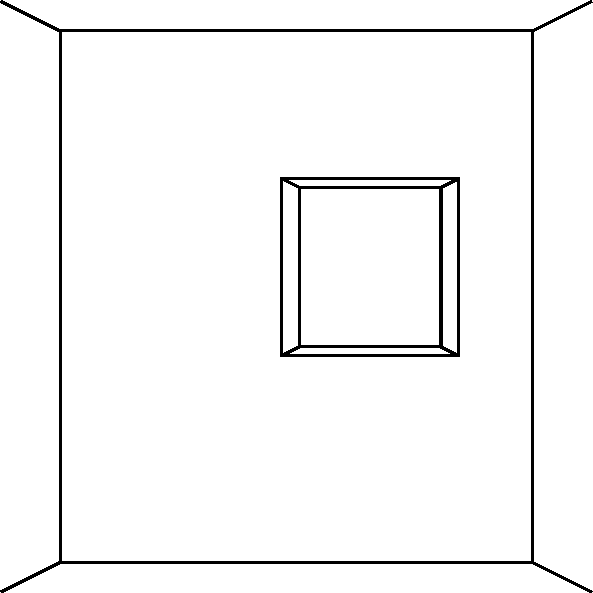
\includegraphics{figures/daytime/daytime.pdf}

}

\subcaption{\label{fig-daytime}}

\end{minipage}%
%
\begin{minipage}{0.04\linewidth}
~\end{minipage}%
%
\begin{minipage}{0.44\linewidth}

\centering{

\captionsetup{labelsep=none}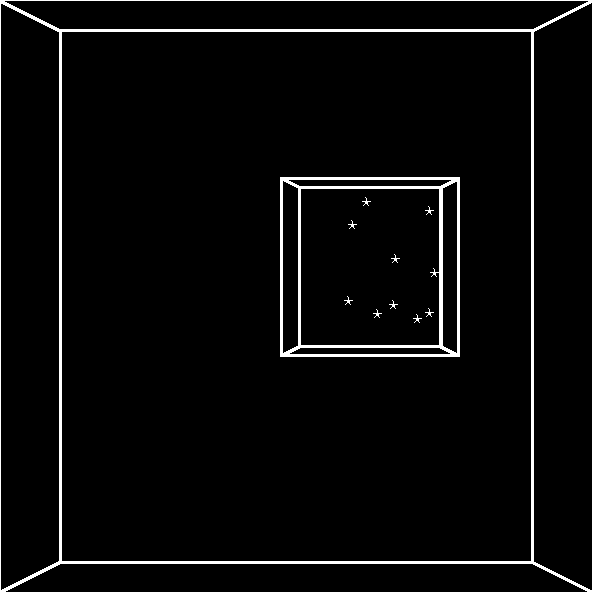
\includegraphics{figures/nighttime/nighttime.pdf}

}

\subcaption{\label{fig-nighttime}}

\end{minipage}%
%
\begin{minipage}{0.04\linewidth}
~\end{minipage}%

\caption{\label{fig-setup}External light passing through a window allow
us to differentiate the window from the surrounding wall. (a) During the
day the bright sunlight allows us to fully characterize the window
geometry but (b) during a moonless night we are limited to starlight
which only partially informs the window geometry.}

\end{figure}%

While the starlight does not allow us to completely determine the
geometry of the window it does provide some information. Our goal is to
infer the window geometries that are consistent with the stars visible
on a given night.

To that end let's set up a coordinate system that describes the geometry
of the room, including both the wall and the window
(Figure~\ref{fig-coordinate-system}). Let's say that we do know that the
height and width of the wall are both \(2 \, L = 6\) meters. We can then
denote the left, right, bottom, and top edges of the window with the
variables \(l\), \(r\), \(b\), and \(t\) respectively.

\begin{figure}

\centering{

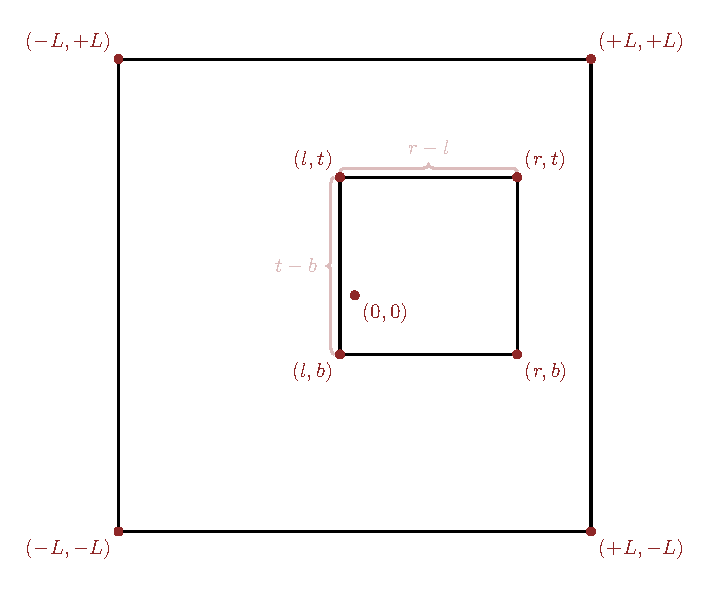
\includegraphics[width=0.5\textwidth,height=\textheight]{figures/coordinate_system/coordinate_system.pdf}

}

\caption{\label{fig-coordinate-system}A natural coordinate system for
this problem is centered on the center of the wall. The left \(l\),
right \(r\), bottom \(b\), and top \(t\) edges of the window can then be
described by distances from this center.}

\end{figure}%

\section{The Observational Model}\label{the-observational-model}

The data generating process here is relatively straightforward. Given a
collection of stars we observe the positions of the stars that fall
within the breadth of the window. More formally we have a
\href{https://betanalpha.github.io/assets/chapters_html/modeling_selection.html}{selection
process} with a latent distribution of star positions and a
deterministic selection function that rejects all stars that are
obscured by the wall.

Firstly let's assume that the horizontal and vertical positions of each
star that we could possibly see are uniformly distributed across the
total breadth of the wall, \[
p(x, y) = \text{uniform}(x \mid -L, +L) \, \text{uniform}(y \mid -L, +L).
\]

The wall then defines a deterministic selection function for a star
being observed, \[
p(z = 1 \mid x, y, l, r, b, t) = I_{(l, r)}(x) \, I_{(b, t)}(y).
\]

Finally the observed star positions are modeled as \begin{align*}
p(x, y &\mid z = 1, l, r, b, t)
\\
&=
\frac{ p(x, y) \, p(z = 1 \mid x, y) }
{ \int \mathrm{d} x \, \mathrm{d} y \, p(x, y) \, p(z = 1 \mid x, y) }
\\
&=
\frac{ \text{uniform}(x \mid -L, +L) \, \text{uniform}(y \mid -L, +L) \,
  I_{(l, r)}(x) \, I_{(b, t)}(y) }
{ \int \mathrm{d} x \, \mathrm{d} y \,
  \text{uniform}(x \mid -L, +L) \, \text{uniform}(y \mid -L, +L) \,
  I_{(l, r)}(x) \, I_{(b, t)}(y) }
\\
&=
\frac{ \text{uniform}(x \mid -L, +L) \, I_{(l, r)}(x) }
{ \int \mathrm{d} x \, \text{uniform}(x \mid -L, +L) \, I_{(l, r)}(x) } \,
\frac{ \text{uniform}(y \mid -L, +L) \, I_{(b, t)}(y) }
{ \int \mathrm{d} y \, \text{uniform}(y \mid -L, +L) \, I_{(b, t)}(y) }
\end{align*}

To simplify this further we'll need to take advantage of two facts.
First the uniform probability density function is defined by an
indicator function of its own, \[
\text{uniform}(z \mid a, b) = \frac{ I_{(a, b)}(z) }{ | b - a | }.
\] Second the product of two interval indicator functions is given by
the indicator function of the intersection of the two intervals, \[
I_{(a, b)}(z) \, I_{(c, d)}(z) = I_{(a, b) \cap (c, d)}(z).
\] Putting these two properties together gives \begin{align*}
\text{uniform}(z \mid a, b) \, I_{(c, d)}(z)
&=
\frac{ I_{(a, b)}(z) }{ | b - a | } \, I_{(c, d)}(z)
\\
&=
\frac{ I_{(a, b)}(z) \, I_{(c, d)}(z) }{ | b - a | }
\\
&=
\frac{ I_{(a, b) \cap (c, d)}(z) }{ | b - a | }.
\end{align*}

Because \((l, r) \subset (-L, +L)\) we have \[
(-L, +L) \cap (l, r) = (l, r)
\] and consequently \begin{align*}
\text{uniform}(x \mid -L, +L) \, I_{(l, r)}(x)
&=
\frac{ I_{(-L, +L) \cap (l, r)}(x) }{ 2 L }
\\
&=
\frac{ I_{(l, r)}(x) }{ 2 L }.
\end{align*} Similarly \[
\text{uniform}(x \mid -L, +L) \, I_{(b, t)}(y) = \frac{ I_{(b, t)}(y) }{ 2 L }.
\]

Substituting these two results into the observational model for a single
star finally gives \begin{align*}
p(x, y &\mid z = 1, l, r, b, t)
\\
&=
\frac{ \text{uniform}(x \mid -L, +L) \, I_{(l, r)}(x) }
{ \int \mathrm{d} x \, \text{uniform}(x \mid -L, +L) \, I_{(l, r)}(x) } \,
\frac{ \text{uniform}(y \mid -L, +L) \, I_{(b, t)}(y) }
{ \int \mathrm{d} y \, \text{uniform}(y \mid -L, +L) \, I_{(b, t)}(y) }
\\
&=
\frac{ I_{(l, r)}(x) / (2L) }{ \int \mathrm{d} x \, I_{(l, r)}(x) / (2L) } \,
\frac{ I_{(b, t)}(y) / (2L) }{ \int \mathrm{d} y \, I_{(b, t)}(y) / (2L) }
\\
&=
\frac{ I_{(l, r)}(x) }{ \int \mathrm{d} x \, I_{(l, r)}(x) } \,
\frac{ I_{(b, t)}(y) }{ \int \mathrm{d} y \, I_{(b, t)}(y) }
\\
&=
\frac{ I_{(l, r)}(x) }{ | r - l | } \,
\frac{ I_{(b, t)}(y) }{ | t - b | }.
\end{align*}

When we observe \(N\) total stars with \emph{independent} positions
\((x_{n}, y_{n})\) the total observational model becomes \begin{align*}
p(x_{1}, y_{1}, \ldots, x_{N}, y_{N} \mid z = 1, l, r, b, t)
&=
\prod_{n = 1}^{N} \frac{ I_{(l, r)}(x_{n}) }{ | r - l | } \,
                  \frac{ I_{(b, t)}(y_{n}) }{ | t - b | }
\\
&=
\frac{ \prod_{n = 1}^{N} I_{(l, r)}(x_{n}) \, I_{(b, t)}(y_{n}) }
{ | r - l |^{N} \, | t - b |^{N} }.
\end{align*}

\section{The Likelihood Function}\label{the-likelihood-function}

In theory the likelihood function for the window geometry is given by
evaluating the observational probability density function on a set
observed positions, \begin{align*}
\mathcal{L}(l, r, b, t)
&\propto
p(\tilde{x}_{1}, \tilde{y}_{1}, \ldots, \tilde{x}_{N}, \tilde{y}_{N} \mid
  z = 1, l, r, b, t)
\\
&\propto
\frac{
  \prod_{n = 1}^{N} I_{(l, r)}( \tilde{x}_{n}) \, I_{(b, t)}( \tilde{y}_{n})
}
{
  | r - l |^{N} \, | t - b |^{N}
}.
\end{align*} This likelihood function, however, appears to be a bit
ungainly to use in practice because of the many discontinuities
introduced by all of those indicator functions.

Fortunately this issue is largely an illusion of how we have written the
likelihood function here; most of these indicator functions are in fact
redundant and can be removed entirely. With a little bit of work we can
eliminate these redundancies and simplify the likelihood function into a
form that is much easier to wield in practice.

The key to this simplification is to manipulate the indicator functions
over the varying star positions into indicator functions over the common
window position parameters. In general the indicator function
\(I_{(a, b)}(z)\) gives non-zero outputs only when \[
a < z < b.
\] This sequence of inequalities, however, can also be written as three
separate inequalities, \begin{align*}
a &< z
\\
z &< b
\\
a &< b.
\end{align*} In turn these separate inequalities define three indicator
functions for the interval parameters \(a\) and \(b\), \begin{align*}
I_{(-\infty, z)}(a)
\\
I_{(z, +\infty)}(b)
\\
I_{(-\infty, b)}(a).
\end{align*} Consequently we can we can always write the indicator
function \(I_{(a, b)}(z)\) as a product of these three indicator
functions, \[
I_{(a, b)}(z)
=
I_{(-\infty, z)}(a) \, I_{(z, +\infty)}(b) \, I_{(-\infty, b)}(a).
\] Again the first indicator function ensures that \(a\) is less than
\(z\), the second indicator function ensures that \(b\) is larger than
\(z\), and the third indicator function ensures that \(a\) is less than
\(b\) which is required for \((a, b)\) to be a well-defined interval.

This decomposition then allow us to write any product of indicator
functions evaluations as \begin{align*}
\prod_{n = 1}^{N}
I_{(a, b)}(z_{n})
&=
\prod_{n = 1}^{N}
I_{(-\infty, z_{n})}(a) \, I_{(z_{n}, +\infty)}(b) \, I_{(-\infty, b)}(a)
\\
&=
\left[ \prod_{n = 1}^{N} I_{(-\infty, z_{n})}(a) \right] \,
\left[ \prod_{n = 1}^{N} I_{(z_{n}, +\infty)}(b) \right] \,
\left[ \prod_{n = 1}^{N} I_{(-\infty, b)}(a) \right]
\\
&=
\left[ \prod_{n = 1}^{N} I_{(-\infty, z_{n})}(a) \right] \,
\left[ \prod_{n = 1}^{N} I_{(z_{n}, +\infty)}(b) \right] \,
\left( I_{(-\infty, b)}(a) \right)^{N}
\\
&=
\left[ \prod_{n = 1}^{N} I_{(-\infty, z_{n})}(a) \right] \,
\left[ \prod_{n = 1}^{N} I_{(z_{n}, +\infty)}(b) \right] \,
I_{(-\infty, b)}(a).
\end{align*}

Now the overlap of the intervals \((-\infty, z_{n})\) is completely
determined by the smallest \(z_{n}\), \[
\bigcap_{n = 1}^{N} (-\infty, z_{n}) = (-\infty, \min(z_{n})).
\] Consequently the first product reduces to \begin{align*}
\prod_{n = 1}^{N} I_{(-\infty, z_{n})}(a)
&=
I_{ \cap_{n = 1}^{N} (-\infty, z_{n}) }(a)
\\
&=
I_{ (-\infty, \min(z_{n})) }(a).
\end{align*} Similarly \[
\bigcap_{n = 1}^{N} (z_{n}, +\infty) = (\max(z_{n}), +\infty).
\] and \begin{align*}
\prod_{n = 1}^{N} I_{(z_{n}, +\infty)}(b)
&=
I_{ \cap_{n = 1}^{N} (z_{n}, +\infty) }(b)
\\
&=
I_{ (\max(z_{n}), +\infty) }(b).
\end{align*}

This allows us to replace all of those indicator functions with just
three indicator functions, \begin{align*}
\prod_{n = 1}^{N}
I_{(a, b)}(z_{n})
&=
\left[ \prod_{n = 1}^{N} I_{(-\infty, z_{n})}(a) \right] \,
\left[ \prod_{n = 1}^{N} I_{(z_{n}, +\infty)}(b) \right] \,
I_{(-\infty, b)}(a)
\\
&=
I_{ (-\infty, \min(z_{n})) }(a) \,
I_{ (\max(z_{n}), +\infty) }(b) \,
I_{(-\infty, b)}(a).
\end{align*} For real-valued \(z_{n}\) ties will occur with probability
zero and we will have \[
\min(z_{n}) < \max(z_{n})
\] with probability one so that the last indicator function is also
redundant. Consequently we can write \[
\prod_{n = 1}^{N}
I_{(a, b)}(z_{n})
=
I_{ (-\infty, \min(z_{n})) }(a) \,
I_{ (\max(z_{n}), +\infty) }(b).
\]

Applying this result twice our likelihood function takes on the much
simpler form \begin{align*}
\mathcal{L}(l, r, b, t)
&\propto
\frac{
  \prod_{n = 1}^{N} I_{(l, r)}( \tilde{x}_{n}) \, I_{(b, t)}( \tilde{y}_{n})
}
{
  | r - l |^{N} \, | t - b |^{N}
}
\\
&\propto
\frac{
  \prod_{n = 1}^{N} I_{(l, r)}( \tilde{x}_{n}) \,
  \prod_{n = 1}^{N} I_{(b, t)}( \tilde{y}_{n})
}
{
  | r - l |^{N} \, | t - b |^{N}
}
\\
&\propto \;\,
\frac{
  I_{ (-\infty, \min(\tilde{x}_{n})) }(l) \,
  I_{ (\max(\tilde{x}_{n}), +\infty) }(r)
}
{
  | r - l |^{N}
}
\\
&\quad \cdot
\frac{
  I_{ (-\infty, \min(\tilde{y}_{n})) }(b) \,
  I_{ (\max(\tilde{y}_{n}), +\infty) }(t)
}
{
  | t - b |^{N}
}.
\end{align*} The first indicator function keeps the left window boundary
below all observed \(x\) positions while the second indicator function
keeps the right window boundary above all observed \(y\) positions.
Similarly the last two indicator functions ensure that the bottom window
boundary is below, and the top window boundary is above, all observed
\(y\) positions. As the number of observations \(N\) grows the
denominator pulls the likelihood function closer and closer to the
minimum and maximum \(x\) and \(y\) positions.

Because the likelihood function can always be written in terms of
\(\min(\tilde{x}_{n})\), \(\max(\tilde{x}_{n})\),
\(\min(\tilde{y}_{n})\), and \(\max(\tilde{y}_{n})\) regardless of what
the individual positions are, these extreme values are \emph{sufficient
statistics} for this particular observational model.

\section{Bayesian Inference}\label{bayesian-inference}

This simplified likelihood function is straightforward to implement in
\texttt{Stan}, allowing us to readily quantify posterior inferences for
the window geometry given observed star positions.

\subsection{Setup}\label{setup}

As always we begin by setting up our local \texttt{R} environment.

\begin{Shaded}
\begin{Highlighting}[]
\FunctionTok{par}\NormalTok{(}\AttributeTok{family=}\StringTok{"serif"}\NormalTok{, }\AttributeTok{las=}\DecValTok{1}\NormalTok{, }\AttributeTok{bty=}\StringTok{"l"}\NormalTok{,}
    \AttributeTok{cex.axis=}\DecValTok{1}\NormalTok{, }\AttributeTok{cex.lab=}\DecValTok{1}\NormalTok{, }\AttributeTok{cex.main=}\DecValTok{1}\NormalTok{,}
    \AttributeTok{xaxs=}\StringTok{"i"}\NormalTok{, }\AttributeTok{yaxs=}\StringTok{"i"}\NormalTok{, }\AttributeTok{mar =} \FunctionTok{c}\NormalTok{(}\DecValTok{5}\NormalTok{, }\DecValTok{5}\NormalTok{, }\DecValTok{3}\NormalTok{, }\DecValTok{5}\NormalTok{))}

\NormalTok{c\_light }\OtherTok{\textless{}{-}} \FunctionTok{c}\NormalTok{(}\StringTok{"\#DCBCBC"}\NormalTok{)}
\NormalTok{c\_light\_highlight }\OtherTok{\textless{}{-}} \FunctionTok{c}\NormalTok{(}\StringTok{"\#C79999"}\NormalTok{)}
\NormalTok{c\_mid }\OtherTok{\textless{}{-}} \FunctionTok{c}\NormalTok{(}\StringTok{"\#B97C7C"}\NormalTok{)}
\NormalTok{c\_mid\_highlight }\OtherTok{\textless{}{-}} \FunctionTok{c}\NormalTok{(}\StringTok{"\#A25050"}\NormalTok{)}
\NormalTok{c\_dark }\OtherTok{\textless{}{-}} \FunctionTok{c}\NormalTok{(}\StringTok{"\#8F2727"}\NormalTok{)}
\NormalTok{c\_dark\_highlight }\OtherTok{\textless{}{-}} \FunctionTok{c}\NormalTok{(}\StringTok{"\#7C0000"}\NormalTok{)}

\NormalTok{c\_light\_teal }\OtherTok{\textless{}{-}} \FunctionTok{c}\NormalTok{(}\StringTok{"\#6B8E8E"}\NormalTok{)}
\NormalTok{c\_mid\_teal }\OtherTok{\textless{}{-}} \FunctionTok{c}\NormalTok{(}\StringTok{"\#487575"}\NormalTok{)}
\NormalTok{c\_dark\_teal }\OtherTok{\textless{}{-}} \FunctionTok{c}\NormalTok{(}\StringTok{"\#1D4F4F"}\NormalTok{)}

\FunctionTok{library}\NormalTok{(colormap)}
\NormalTok{disc\_colors }\OtherTok{\textless{}{-}} \FunctionTok{c}\NormalTok{(}\StringTok{"\#FFFFFF"}\NormalTok{, }\StringTok{"\#DCBCBC"}\NormalTok{, }\StringTok{"\#C79999"}\NormalTok{, }\StringTok{"\#B97C7C"}\NormalTok{,}
                 \StringTok{"\#A25050"}\NormalTok{, }\StringTok{"\#8F2727"}\NormalTok{, }\StringTok{"\#7C0000"}\NormalTok{)}
\end{Highlighting}
\end{Shaded}

In particular we'll need to load \texttt{RStan} and my recommended
Hamiltonian Monte Carlo analysis suite.

\begin{Shaded}
\begin{Highlighting}[]
\FunctionTok{library}\NormalTok{(rstan)}
\FunctionTok{rstan\_options}\NormalTok{(}\AttributeTok{auto\_write =} \ConstantTok{TRUE}\NormalTok{)            }\CommentTok{\# Cache compiled Stan programs}
\FunctionTok{options}\NormalTok{(}\AttributeTok{mc.cores =}\NormalTok{ parallel}\SpecialCharTok{::}\FunctionTok{detectCores}\NormalTok{()) }\CommentTok{\# Parallelize chains}
\NormalTok{parallel}\SpecialCharTok{:::}\FunctionTok{setDefaultClusterOptions}\NormalTok{(}\AttributeTok{setup\_strategy =} \StringTok{"sequential"}\NormalTok{)}

\NormalTok{util }\OtherTok{\textless{}{-}} \FunctionTok{new.env}\NormalTok{()}
\FunctionTok{source}\NormalTok{(}\StringTok{\textquotesingle{}stan\_utility\_rstan.R\textquotesingle{}}\NormalTok{, }\AttributeTok{local=}\NormalTok{util)}
\end{Highlighting}
\end{Shaded}

\subsection{Explore Data}\label{explore-data}

Let's start by reading in the observed star positions.

\begin{Shaded}
\begin{Highlighting}[]
\NormalTok{data }\OtherTok{\textless{}{-}} \FunctionTok{read\_rdump}\NormalTok{(}\StringTok{"data/stars.data.R"}\NormalTok{)}
\end{Highlighting}
\end{Shaded}

The observed stars positions imply that the window is situated towards
the top right corner of the wall but the precise edges of the windows
are hard to resolve.

\begin{Shaded}
\begin{Highlighting}[]
\NormalTok{L }\OtherTok{\textless{}{-}} \DecValTok{3}
\FunctionTok{par}\NormalTok{(}\AttributeTok{mfrow=}\FunctionTok{c}\NormalTok{(}\DecValTok{1}\NormalTok{, }\DecValTok{1}\NormalTok{), }\AttributeTok{mar=}\FunctionTok{c}\NormalTok{(}\DecValTok{0}\NormalTok{, }\DecValTok{0}\NormalTok{, }\DecValTok{0}\NormalTok{, }\DecValTok{0}\NormalTok{))}

\FunctionTok{plot}\NormalTok{(}\DecValTok{0}\NormalTok{, }\AttributeTok{type=}\StringTok{\textquotesingle{}n\textquotesingle{}}\NormalTok{,}
     \AttributeTok{xlim=}\FunctionTok{c}\NormalTok{(}\SpecialCharTok{{-}}\NormalTok{L, }\SpecialCharTok{+}\NormalTok{L), }\AttributeTok{ylim=}\FunctionTok{c}\NormalTok{(}\SpecialCharTok{{-}}\NormalTok{L, }\SpecialCharTok{+}\NormalTok{L),}
     \AttributeTok{axes=}\ConstantTok{FALSE}\NormalTok{, }\AttributeTok{ann=}\ConstantTok{FALSE}\NormalTok{)}
\FunctionTok{rect}\NormalTok{(}\SpecialCharTok{{-}}\NormalTok{L, }\SpecialCharTok{{-}}\NormalTok{L, }\SpecialCharTok{+}\NormalTok{L, L, }\AttributeTok{col =} \StringTok{"black"}\NormalTok{)}
\FunctionTok{points}\NormalTok{(data}\SpecialCharTok{$}\NormalTok{xs, data}\SpecialCharTok{$}\NormalTok{ys, }\AttributeTok{col=}\StringTok{"white"}\NormalTok{, }\AttributeTok{pch=}\DecValTok{8}\NormalTok{)}
\end{Highlighting}
\end{Shaded}

\includegraphics{window_inference_files/figure-pdf/unnamed-chunk-6-1.pdf}

\subsection{Quantify Posterior
Distribution}\label{quantify-posterior-distribution}

In addition to the requirement of a positive window size, \begin{align*}
l &< r
\\
b &< t,
\end{align*} the window geometry is constrained by the wall geometry,
\begin{align*}
-L &< l < +L
\\
-L &< r < +L
\\
-L &< b < +L
\\
-L &< t < +L.
\end{align*}

If we don't have any additional information about the position of the
window then our domain expertise is captured by the uniform prior
density function subject to these constraints, \begin{align*}
p(l, r, b, t)
&=
p(l, r) \, p(b, t)
\\
&=\;\,
\text{uniform}(l \mid -L, +L) \, \text{uniform}(r \mid l, +L)
\\
&\quad \cdot
\text{uniform}(b \mid -L, +L) \, \text{uniform}(t \mid b, +L)
\end{align*}

With this prior model the posterior density function completely
decouples into independent posterior density functions for each of the
two directions, \begin{align*}
p(l, r, b, t &\mid
  \tilde{x}_{1}, \tilde{y}_{1}, \ldots, \tilde{x}_{N}, \tilde{y}_{N})
\\
&\propto
p(\tilde{x}_{1}, \tilde{y}_{1}, \ldots, \tilde{x}_{N}, \tilde{y}_{N}) \mid
  l, r, b, t) \,
p(l, r, b, t)
\\
&\propto \;
\frac{
  I_{ (-\infty, \min(\tilde{x}_{n})) }(l) \,
  I_{ (\max(\tilde{x}_{n}), +\infty) }(r)
}
{
  | r - l |^{N}
} \,
\\
&\quad \cdot
\frac{
  I_{ (-\infty, \min(\tilde{y}_{n})) }(b) \,
  I_{ (\max(\tilde{y}_{n}), +\infty) }(t)
}
{
  | t - b |^{N}
} \,
\\
&\quad \cdot
\text{uniform}(l \mid -L, +L) \, \text{uniform}(r \mid l, +L)
\\
&\quad \cdot
\text{uniform}(b \mid -L, +L) \, \text{uniform}(t \mid b, +L)
\\
&\propto \;
\frac{
  I_{ (-\infty, \min(\tilde{x}_{n})) }(l) \,
  I_{ (\max(\tilde{x}_{n}), +\infty) }(r) \,
}
{ | r - l |^{N} }
\\
&\quad \cdot
\text{uniform}(l \mid -L, +L) \, \text{uniform}(r \mid l, +L)
\\
&\quad \cdot
\frac{
  I_{ (-\infty, \min(\tilde{y}_{n})) }(b) \,
  I_{ (\max(\tilde{y}_{n}), +\infty) }(t)
}
{ | t - b |^{N} }
\\
&\quad \cdot
\text{uniform}(b \mid -L, +L) \, \text{uniform}(t \mid b, +L)
\\
&\propto \;\,
p(l, r \mid \tilde{x}_{1}, \tilde{y}_{1}, \ldots, \tilde{x}_{N}, \tilde{y}_{N})
\\
&\quad \cdot
p(b, t \mid \tilde{x}_{1}, \tilde{y}_{1}, \ldots, \tilde{x}_{N}, \tilde{y}_{N}).
\end{align*}

In particular we can immediately pushforward the four-dimensional
posterior density function into two-dimensional, marginal posterior
density functions for the horizontal and vertical geometries,
\begin{align*}
p(l, r \mid \tilde{x}_{1}, \tilde{y}_{1}, \ldots, \tilde{x}_{N}, \tilde{y}_{N})
&\propto \;
\frac{
  I_{ (-\infty, \min(\tilde{x}_{n})) }(l) \,
  I_{ (\max(\tilde{x}_{n}), +\infty) }(r) \,
}
{ | r - l |^{N} }
\\
&\quad \cdot
\text{uniform}(l \mid -L, +L) \, \text{uniform}(r \mid l, +L)
\end{align*} and \begin{align*}
p(b, t \mid \tilde{x}_{1}, \tilde{y}_{1}, \ldots, \tilde{x}_{N}, \tilde{y}_{N})
&\propto \;
\frac{
  I_{ (-\infty, \min(\tilde{y}_{n})) }(b) \,
  I_{ (\max(\tilde{y}_{n}), +\infty) }(t)
}
{ | t - b |^{N} }
\\
&\quad \cdot
\text{uniform}(b \mid -L, +L) \, \text{uniform}(t \mid b, +L).
\end{align*} Plotting these marginal posterior density functions
demonstrates how our inferences push up against the constraints imposed
by the minimum and maximum star positions.

\begin{Shaded}
\begin{Highlighting}[]
\FunctionTok{par}\NormalTok{(}\AttributeTok{mfrow=}\FunctionTok{c}\NormalTok{(}\DecValTok{1}\NormalTok{, }\DecValTok{2}\NormalTok{), }\AttributeTok{mar=}\FunctionTok{c}\NormalTok{(}\DecValTok{5}\NormalTok{, }\DecValTok{5}\NormalTok{, }\DecValTok{2}\NormalTok{, }\DecValTok{1}\NormalTok{))}

\NormalTok{K }\OtherTok{\textless{}{-}} \DecValTok{200}
\NormalTok{left\_grid }\OtherTok{\textless{}{-}} \FunctionTok{seq}\NormalTok{(}\SpecialCharTok{{-}}\NormalTok{L, }\SpecialCharTok{+}\NormalTok{L, }\DecValTok{2} \SpecialCharTok{*}\NormalTok{ L }\SpecialCharTok{/}\NormalTok{ (K }\SpecialCharTok{{-}} \DecValTok{1}\NormalTok{))}
\NormalTok{right\_grid }\OtherTok{\textless{}{-}} \FunctionTok{seq}\NormalTok{(}\SpecialCharTok{{-}}\NormalTok{L, }\SpecialCharTok{+}\NormalTok{L, }\DecValTok{2} \SpecialCharTok{*}\NormalTok{ L }\SpecialCharTok{/}\NormalTok{ (K }\SpecialCharTok{{-}} \DecValTok{1}\NormalTok{))}

\NormalTok{post\_pds }\OtherTok{\textless{}{-}} \FunctionTok{matrix}\NormalTok{(}\DecValTok{0}\NormalTok{, }\AttributeTok{nrow=}\NormalTok{K, }\AttributeTok{ncol=}\NormalTok{K)}

\ControlFlowTok{for}\NormalTok{ (k }\ControlFlowTok{in} \DecValTok{1}\SpecialCharTok{:}\NormalTok{K) \{}
  \ControlFlowTok{for}\NormalTok{ (kk }\ControlFlowTok{in} \DecValTok{1}\SpecialCharTok{:}\NormalTok{K) \{}
    \ControlFlowTok{if}\NormalTok{ (left\_grid[k] }\SpecialCharTok{\textgreater{}} \FunctionTok{min}\NormalTok{(data}\SpecialCharTok{$}\NormalTok{xs)) \{}
\NormalTok{      post\_pds[k, kk] }\OtherTok{\textless{}{-}} \DecValTok{0}
\NormalTok{    \} }\ControlFlowTok{else} \ControlFlowTok{if}\NormalTok{ (right\_grid[kk] }\SpecialCharTok{\textless{}} \FunctionTok{max}\NormalTok{(data}\SpecialCharTok{$}\NormalTok{xs)) \{}
\NormalTok{      post\_pds[k, kk] }\OtherTok{\textless{}{-}} \DecValTok{0}
\NormalTok{    \} }\ControlFlowTok{else}\NormalTok{ \{}
\NormalTok{      post\_pds[k, kk] }\OtherTok{\textless{}{-}}\NormalTok{ (right\_grid[kk] }\SpecialCharTok{{-}}\NormalTok{ left\_grid[k])}\SpecialCharTok{**}\NormalTok{(}\SpecialCharTok{{-}}\NormalTok{data}\SpecialCharTok{$}\NormalTok{N)}
\NormalTok{    \}}
\NormalTok{  \}}
\NormalTok{\}}

\NormalTok{disc\_colors }\OtherTok{\textless{}{-}} \FunctionTok{c}\NormalTok{(}\StringTok{"\#FFFFFF"}\NormalTok{, }\StringTok{"\#DCBCBC"}\NormalTok{, }\StringTok{"\#C79999"}\NormalTok{, }\StringTok{"\#B97C7C"}\NormalTok{,}
                 \StringTok{"\#A25050"}\NormalTok{, }\StringTok{"\#8F2727"}\NormalTok{, }\StringTok{"\#7C0000"}\NormalTok{)}
\NormalTok{cont\_colors }\OtherTok{\textless{}{-}} \FunctionTok{colormap}\NormalTok{(}\AttributeTok{colormap=}\NormalTok{disc\_colors, }\AttributeTok{nshades=}\DecValTok{100}\NormalTok{)}

\FunctionTok{image}\NormalTok{(left\_grid, right\_grid, post\_pds, }\AttributeTok{col=}\FunctionTok{rev}\NormalTok{(cont\_colors),}
      \AttributeTok{xlim=}\FunctionTok{c}\NormalTok{(}\SpecialCharTok{{-}}\NormalTok{L, }\SpecialCharTok{+}\NormalTok{L), }\AttributeTok{xlab=}\FunctionTok{c}\NormalTok{(}\StringTok{"Left"}\NormalTok{), }\AttributeTok{ylim=}\FunctionTok{c}\NormalTok{(}\SpecialCharTok{{-}}\NormalTok{L, }\SpecialCharTok{+}\NormalTok{L), }\AttributeTok{ylab=}\FunctionTok{c}\NormalTok{(}\StringTok{"Right"}\NormalTok{),}
      \AttributeTok{main=}\StringTok{"Horizontal Dimensions"}\NormalTok{)}
\FunctionTok{abline}\NormalTok{(}\AttributeTok{v=}\FunctionTok{min}\NormalTok{(data}\SpecialCharTok{$}\NormalTok{xs), }\AttributeTok{lty=}\DecValTok{2}\NormalTok{, }\AttributeTok{lwd=}\DecValTok{2}\NormalTok{, }\AttributeTok{col=}\StringTok{"\#DDDDDD"}\NormalTok{)}
\FunctionTok{text}\NormalTok{(}\FloatTok{0.75}\NormalTok{, }\SpecialCharTok{{-}}\FloatTok{2.75}\NormalTok{, }\StringTok{"min(x\_n)"}\NormalTok{, }\AttributeTok{col=}\StringTok{"\#DDDDDD"}\NormalTok{)}
\FunctionTok{abline}\NormalTok{(}\AttributeTok{h=}\FunctionTok{max}\NormalTok{(data}\SpecialCharTok{$}\NormalTok{xs), }\AttributeTok{lty=}\DecValTok{2}\NormalTok{, }\AttributeTok{lwd=}\DecValTok{2}\NormalTok{, }\AttributeTok{col=}\StringTok{"\#DDDDDD"}\NormalTok{)}
\FunctionTok{text}\NormalTok{(}\DecValTok{2}\NormalTok{,  }\FloatTok{1.25}\NormalTok{, }\StringTok{"max(x\_n)"}\NormalTok{, }\AttributeTok{col=}\StringTok{"\#DDDDDD"}\NormalTok{)}

\NormalTok{K }\OtherTok{\textless{}{-}} \DecValTok{200}
\NormalTok{bottom\_grid }\OtherTok{\textless{}{-}} \FunctionTok{seq}\NormalTok{(}\SpecialCharTok{{-}}\NormalTok{L, }\SpecialCharTok{+}\NormalTok{L, }\DecValTok{2} \SpecialCharTok{*}\NormalTok{ L }\SpecialCharTok{/}\NormalTok{ (K }\SpecialCharTok{{-}} \DecValTok{1}\NormalTok{))}
\NormalTok{top\_grid }\OtherTok{\textless{}{-}} \FunctionTok{seq}\NormalTok{(}\SpecialCharTok{{-}}\NormalTok{L, }\SpecialCharTok{+}\NormalTok{L, }\DecValTok{2} \SpecialCharTok{*}\NormalTok{ L }\SpecialCharTok{/}\NormalTok{ (K }\SpecialCharTok{{-}} \DecValTok{1}\NormalTok{))}

\NormalTok{post\_pds }\OtherTok{\textless{}{-}} \FunctionTok{matrix}\NormalTok{(}\DecValTok{0}\NormalTok{, }\AttributeTok{nrow=}\NormalTok{K, }\AttributeTok{ncol=}\NormalTok{K)}

\ControlFlowTok{for}\NormalTok{ (k }\ControlFlowTok{in} \DecValTok{1}\SpecialCharTok{:}\NormalTok{K) \{}
  \ControlFlowTok{for}\NormalTok{ (kk }\ControlFlowTok{in} \DecValTok{1}\SpecialCharTok{:}\NormalTok{K) \{}
    \ControlFlowTok{if}\NormalTok{ (bottom\_grid[k] }\SpecialCharTok{\textgreater{}} \FunctionTok{min}\NormalTok{(data}\SpecialCharTok{$}\NormalTok{ys)) \{}
\NormalTok{      post\_pds[k, kk] }\OtherTok{\textless{}{-}} \DecValTok{0}
\NormalTok{    \} }\ControlFlowTok{else} \ControlFlowTok{if}\NormalTok{ (top\_grid[kk] }\SpecialCharTok{\textless{}} \FunctionTok{max}\NormalTok{(data}\SpecialCharTok{$}\NormalTok{ys)) \{}
\NormalTok{      post\_pds[k, kk] }\OtherTok{\textless{}{-}} \DecValTok{0}
\NormalTok{    \} }\ControlFlowTok{else}\NormalTok{ \{}
\NormalTok{      post\_pds[k, kk] }\OtherTok{\textless{}{-}}\NormalTok{ (top\_grid[kk] }\SpecialCharTok{{-}}\NormalTok{ bottom\_grid[k])}\SpecialCharTok{**}\NormalTok{(}\SpecialCharTok{{-}}\NormalTok{data}\SpecialCharTok{$}\NormalTok{N)}
\NormalTok{    \}}
\NormalTok{  \}}
\NormalTok{\}}

\FunctionTok{image}\NormalTok{(bottom\_grid, top\_grid, post\_pds, }\AttributeTok{col=}\FunctionTok{rev}\NormalTok{(cont\_colors),}
      \AttributeTok{xlim=}\FunctionTok{c}\NormalTok{(}\SpecialCharTok{{-}}\NormalTok{L, }\SpecialCharTok{+}\NormalTok{L), }\AttributeTok{xlab=}\FunctionTok{c}\NormalTok{(}\StringTok{"Bottom"}\NormalTok{), }\AttributeTok{ylim=}\FunctionTok{c}\NormalTok{(}\SpecialCharTok{{-}}\NormalTok{L, }\SpecialCharTok{+}\NormalTok{L), }\AttributeTok{ylab=}\FunctionTok{c}\NormalTok{(}\StringTok{"Top"}\NormalTok{),}
      \AttributeTok{main=}\StringTok{"Vertical Dimensions"}\NormalTok{)}
\FunctionTok{abline}\NormalTok{(}\AttributeTok{v=}\FunctionTok{min}\NormalTok{(data}\SpecialCharTok{$}\NormalTok{ys), }\AttributeTok{lty=}\DecValTok{2}\NormalTok{, }\AttributeTok{lwd=}\DecValTok{2}\NormalTok{, }\AttributeTok{col=}\StringTok{"\#DDDDDD"}\NormalTok{)}
\FunctionTok{text}\NormalTok{(}\DecValTok{1}\NormalTok{, }\SpecialCharTok{{-}}\FloatTok{2.75}\NormalTok{, }\StringTok{"min(y\_n)"}\NormalTok{, }\AttributeTok{col=}\StringTok{"\#DDDDDD"}\NormalTok{)}
\FunctionTok{abline}\NormalTok{(}\AttributeTok{h=}\FunctionTok{max}\NormalTok{(data}\SpecialCharTok{$}\NormalTok{ys), }\AttributeTok{lty=}\DecValTok{2}\NormalTok{, }\AttributeTok{lwd=}\DecValTok{2}\NormalTok{, }\AttributeTok{col=}\StringTok{"\#DDDDDD"}\NormalTok{)}
\FunctionTok{text}\NormalTok{(}\DecValTok{2}\NormalTok{,  }\FloatTok{1.5}\NormalTok{, }\StringTok{"max(y\_n)"}\NormalTok{, }\AttributeTok{col=}\StringTok{"\#DDDDDD"}\NormalTok{)}
\end{Highlighting}
\end{Shaded}

\includegraphics{window_inference_files/figure-pdf/unnamed-chunk-7-1.pdf}

If we want to extract additional information out of our posterior
distribution then we'll need to resort to posterior expectation values
and the Markov chain Monte Carlo estimators that approximate them.

The summary statistics \(\min(\tilde{x}_{n})\), \(\max(\tilde{x}_{n})\),
\(\min(\tilde{y}_{n})\), and \(\max(\tilde{y}_{n})\) make for natural
retrodictive summaries here. Conveniently we can compute the posterior
predictive summary statistics directly in the
\texttt{generated\ quantities} block.

\begin{codelisting}

\caption{\texttt{fit\textbackslash\_window.stan}}

\begin{Shaded}
\begin{Highlighting}[]
\KeywordTok{data}\NormalTok{ \{}
  \DataTypeTok{int}\NormalTok{\textless{}}\KeywordTok{lower}\NormalTok{=}\DecValTok{1}\NormalTok{\textgreater{} N; }\CommentTok{// Number of observations}
  \DataTypeTok{real}\NormalTok{ xs[N];     }\CommentTok{// Observed x positions (m)}
  \DataTypeTok{real}\NormalTok{ ys[N];     }\CommentTok{// Observed y positions (m)}
\NormalTok{\}}

\KeywordTok{transformed data}\NormalTok{ \{}
  \DataTypeTok{real}\NormalTok{ L = }\DecValTok{3}\NormalTok{; }\CommentTok{// Maximum size (m)}

  \CommentTok{// Sufficient statistics}
  \DataTypeTok{real}\NormalTok{ min\_x = min(xs);}
  \DataTypeTok{real}\NormalTok{ max\_x = max(xs);}
  \DataTypeTok{real}\NormalTok{ min\_y = min(ys);}
  \DataTypeTok{real}\NormalTok{ max\_y = max(ys);}
\NormalTok{\}}

\KeywordTok{parameters}\NormalTok{ \{}
  \DataTypeTok{real}\NormalTok{\textless{}}\KeywordTok{lower}\NormalTok{={-}L, }\KeywordTok{upper}\NormalTok{=min\_x\textgreater{} left;   }\CommentTok{// Position of left window edge (m)}
  \DataTypeTok{real}\NormalTok{\textless{}}\KeywordTok{lower}\NormalTok{=max\_x, }\KeywordTok{upper}\NormalTok{=+L\textgreater{} right;  }\CommentTok{// Position of right window edge (m)}
  \DataTypeTok{real}\NormalTok{\textless{}}\KeywordTok{lower}\NormalTok{={-}L, }\KeywordTok{upper}\NormalTok{=min\_y\textgreater{} bottom; }\CommentTok{// Position of bottom window edge (m)}
  \DataTypeTok{real}\NormalTok{\textless{}}\KeywordTok{lower}\NormalTok{=max\_y, }\KeywordTok{upper}\NormalTok{=+L\textgreater{} top;    }\CommentTok{// Position of top window edge (m)}
\NormalTok{\}}

\KeywordTok{model}\NormalTok{ \{}
  \CommentTok{// Implicit uniform prior density function within boundaries}
  
  \CommentTok{// Observational model}
  \KeywordTok{target +=}\NormalTok{ {-} N * ( log(right {-} left) + log(top {-} bottom));}
\NormalTok{\}}

\KeywordTok{generated quantities}\NormalTok{ \{}
  \DataTypeTok{real}\NormalTok{ min\_x\_pred;}
  \DataTypeTok{real}\NormalTok{ max\_x\_pred;}
  \DataTypeTok{real}\NormalTok{ min\_y\_pred;}
  \DataTypeTok{real}\NormalTok{ max\_y\_pred;}
\NormalTok{  \{}
    \DataTypeTok{real}\NormalTok{ xs\_pred[N];}
    \DataTypeTok{real}\NormalTok{ ys\_pred[N];}
    \ControlFlowTok{for}\NormalTok{ (n }\ControlFlowTok{in} \DecValTok{1}\NormalTok{:N) \{}
\NormalTok{      xs\_pred[n] = uniform\_rng(left, right);}
\NormalTok{      ys\_pred[n] = uniform\_rng(bottom, top);}
\NormalTok{    \}}

\NormalTok{    min\_x\_pred = min(xs\_pred);}
\NormalTok{    max\_x\_pred = max(xs\_pred);}
\NormalTok{    min\_y\_pred = min(ys\_pred);}
\NormalTok{    max\_y\_pred = max(ys\_pred);}
\NormalTok{  \}}
\NormalTok{\}}
\end{Highlighting}
\end{Shaded}

\end{codelisting}

\begin{Shaded}
\begin{Highlighting}[]
\NormalTok{fit }\OtherTok{\textless{}{-}} \FunctionTok{stan}\NormalTok{(}\AttributeTok{file=}\StringTok{"stan\_programs/fit\_window.stan"}\NormalTok{,}
            \AttributeTok{data=}\NormalTok{data, }\AttributeTok{seed=}\DecValTok{8438338}\NormalTok{,}
            \AttributeTok{warmup=}\DecValTok{1000}\NormalTok{, }\AttributeTok{iter=}\DecValTok{2024}\NormalTok{, }\AttributeTok{refresh=}\DecValTok{0}\NormalTok{)}
\end{Highlighting}
\end{Shaded}

Conveniently our diagnostics show no serious indications of
computational infidelity.

\begin{Shaded}
\begin{Highlighting}[]
\NormalTok{diagnostics }\OtherTok{\textless{}{-}}\NormalTok{ util}\SpecialCharTok{$}\FunctionTok{extract\_hmc\_diagnostics}\NormalTok{(fit)}
\NormalTok{util}\SpecialCharTok{$}\FunctionTok{check\_all\_hmc\_diagnostics}\NormalTok{(diagnostics)}
\end{Highlighting}
\end{Shaded}

\begin{verbatim}
  All Hamiltonian Monte Carlo diagnostics are consistent with reliable
Markov chain Monte Carlo.
\end{verbatim}

\begin{Shaded}
\begin{Highlighting}[]
\NormalTok{samples }\OtherTok{\textless{}{-}}\NormalTok{ util}\SpecialCharTok{$}\FunctionTok{extract\_expectands}\NormalTok{(fit)}
\NormalTok{base\_samples }\OtherTok{\textless{}{-}}\NormalTok{ util}\SpecialCharTok{$}\FunctionTok{filter\_expectands}\NormalTok{(samples,}
                                       \FunctionTok{c}\NormalTok{(}\StringTok{\textquotesingle{}left\textquotesingle{}}\NormalTok{, }\StringTok{\textquotesingle{}right\textquotesingle{}}\NormalTok{,}
                                         \StringTok{\textquotesingle{}bottom\textquotesingle{}}\NormalTok{, }\StringTok{\textquotesingle{}top\textquotesingle{}}\NormalTok{))}
\NormalTok{util}\SpecialCharTok{$}\FunctionTok{check\_all\_expectand\_diagnostics}\NormalTok{(base\_samples)}
\end{Highlighting}
\end{Shaded}

\begin{verbatim}
left:
  Chain 2: Left tail hat{xi} (0.294) exceeds 0.25!


Large tail hat{xi}s suggest that the expectand might not be
sufficiently integrable.
\end{verbatim}

None of the four summary statistics exhibit any appreciable retrodictive
tension, suggesting that our modeling assumptions are adequate.

\begin{Shaded}
\begin{Highlighting}[]
\FunctionTok{par}\NormalTok{(}\AttributeTok{mfrow=}\FunctionTok{c}\NormalTok{(}\DecValTok{2}\NormalTok{, }\DecValTok{2}\NormalTok{), }\AttributeTok{mar=}\FunctionTok{c}\NormalTok{(}\DecValTok{5}\NormalTok{, }\DecValTok{5}\NormalTok{, }\DecValTok{2}\NormalTok{, }\DecValTok{1}\NormalTok{))}

\NormalTok{util}\SpecialCharTok{$}\FunctionTok{plot\_expectand\_pushforward}\NormalTok{(samples[[}\StringTok{\textquotesingle{}min\_x\_pred\textquotesingle{}}\NormalTok{]], }\DecValTok{25}\NormalTok{, }\StringTok{\textquotesingle{}min\_x\textquotesingle{}}\NormalTok{,}
                                \AttributeTok{baseline=}\FunctionTok{min}\NormalTok{(data}\SpecialCharTok{$}\NormalTok{xs))}
\NormalTok{util}\SpecialCharTok{$}\FunctionTok{plot\_expectand\_pushforward}\NormalTok{(samples[[}\StringTok{\textquotesingle{}max\_x\_pred\textquotesingle{}}\NormalTok{]], }\DecValTok{25}\NormalTok{, }\StringTok{\textquotesingle{}max\_x\textquotesingle{}}\NormalTok{,}
                                \AttributeTok{baseline=}\FunctionTok{max}\NormalTok{(data}\SpecialCharTok{$}\NormalTok{xs))}
\NormalTok{util}\SpecialCharTok{$}\FunctionTok{plot\_expectand\_pushforward}\NormalTok{(samples[[}\StringTok{\textquotesingle{}min\_y\_pred\textquotesingle{}}\NormalTok{]], }\DecValTok{25}\NormalTok{, }\StringTok{\textquotesingle{}min\_y\textquotesingle{}}\NormalTok{,}
                                \AttributeTok{baseline=}\FunctionTok{min}\NormalTok{(data}\SpecialCharTok{$}\NormalTok{ys))}
\NormalTok{util}\SpecialCharTok{$}\FunctionTok{plot\_expectand\_pushforward}\NormalTok{(samples[[}\StringTok{\textquotesingle{}max\_y\_pred\textquotesingle{}}\NormalTok{]], }\DecValTok{25}\NormalTok{, }\StringTok{\textquotesingle{}max\_y\textquotesingle{}}\NormalTok{,}
                                \AttributeTok{baseline=}\FunctionTok{max}\NormalTok{(data}\SpecialCharTok{$}\NormalTok{ys))}
\end{Highlighting}
\end{Shaded}

\includegraphics{window_inference_files/figure-pdf/unnamed-chunk-10-1.pdf}

The Markov chain Monte Carlo fit now allows us to examine marginal
posterior inferences for each individual parameter. All four of the
marginal posterior distributions concentrate towards the hard edge
imposed by the observed summary statistics.

\begin{Shaded}
\begin{Highlighting}[]
\FunctionTok{par}\NormalTok{(}\AttributeTok{mfrow=}\FunctionTok{c}\NormalTok{(}\DecValTok{2}\NormalTok{, }\DecValTok{2}\NormalTok{), }\AttributeTok{mar=}\FunctionTok{c}\NormalTok{(}\DecValTok{5}\NormalTok{, }\DecValTok{5}\NormalTok{, }\DecValTok{2}\NormalTok{, }\DecValTok{1}\NormalTok{))}

\NormalTok{util}\SpecialCharTok{$}\FunctionTok{plot\_expectand\_pushforward}\NormalTok{(samples[[}\StringTok{\textquotesingle{}left\textquotesingle{}}\NormalTok{]], }\DecValTok{25}\NormalTok{,}
                                \StringTok{\textquotesingle{}Left Window Edge\textquotesingle{}}\NormalTok{, }\AttributeTok{flim=}\FunctionTok{c}\NormalTok{(}\SpecialCharTok{{-}}\NormalTok{L, }\SpecialCharTok{+}\NormalTok{L))}
\FunctionTok{abline}\NormalTok{(}\AttributeTok{v=}\FunctionTok{min}\NormalTok{(data}\SpecialCharTok{$}\NormalTok{xs), }\AttributeTok{lty=}\DecValTok{2}\NormalTok{, }\AttributeTok{lwd=}\DecValTok{2}\NormalTok{, }\AttributeTok{col=}\StringTok{"\#DDDDDD"}\NormalTok{)}
\FunctionTok{text}\NormalTok{(}\DecValTok{1}\NormalTok{, }\FloatTok{1.4}\NormalTok{, }\StringTok{"min(x\_n)"}\NormalTok{, }\AttributeTok{col=}\StringTok{"\#DDDDDD"}\NormalTok{)}

\NormalTok{util}\SpecialCharTok{$}\FunctionTok{plot\_expectand\_pushforward}\NormalTok{(samples[[}\StringTok{\textquotesingle{}right\textquotesingle{}}\NormalTok{]], }\DecValTok{25}\NormalTok{,}
                                \StringTok{\textquotesingle{}Right Window Edge\textquotesingle{}}\NormalTok{, }\AttributeTok{flim=}\FunctionTok{c}\NormalTok{(}\SpecialCharTok{{-}}\NormalTok{L, }\SpecialCharTok{+}\NormalTok{L))}
\FunctionTok{abline}\NormalTok{(}\AttributeTok{v=}\FunctionTok{max}\NormalTok{(data}\SpecialCharTok{$}\NormalTok{xs), }\AttributeTok{lty=}\DecValTok{2}\NormalTok{, }\AttributeTok{lwd=}\DecValTok{2}\NormalTok{, }\AttributeTok{col=}\StringTok{"\#DDDDDD"}\NormalTok{)}
\FunctionTok{text}\NormalTok{(}\FloatTok{0.25}\NormalTok{, }\DecValTok{1}\NormalTok{, }\StringTok{"max(x\_n)"}\NormalTok{, }\AttributeTok{col=}\StringTok{"\#DDDDDD"}\NormalTok{)}

\NormalTok{util}\SpecialCharTok{$}\FunctionTok{plot\_expectand\_pushforward}\NormalTok{(samples[[}\StringTok{\textquotesingle{}bottom\textquotesingle{}}\NormalTok{]], }\DecValTok{25}\NormalTok{,}
                                \StringTok{\textquotesingle{}Bottom Window Edge\textquotesingle{}}\NormalTok{, }\AttributeTok{flim=}\FunctionTok{c}\NormalTok{(}\SpecialCharTok{{-}}\NormalTok{L, }\SpecialCharTok{+}\NormalTok{L))}
\FunctionTok{abline}\NormalTok{(}\AttributeTok{v=}\FunctionTok{min}\NormalTok{(data}\SpecialCharTok{$}\NormalTok{ys), }\AttributeTok{lty=}\DecValTok{2}\NormalTok{, }\AttributeTok{lwd=}\DecValTok{2}\NormalTok{, }\AttributeTok{col=}\StringTok{"\#DDDDDD"}\NormalTok{)}
\FunctionTok{text}\NormalTok{(}\DecValTok{1}\NormalTok{, }\FloatTok{1.4}\NormalTok{, }\StringTok{"min(y\_n)"}\NormalTok{, }\AttributeTok{col=}\StringTok{"\#DDDDDD"}\NormalTok{)}

\NormalTok{util}\SpecialCharTok{$}\FunctionTok{plot\_expectand\_pushforward}\NormalTok{(samples[[}\StringTok{\textquotesingle{}top\textquotesingle{}}\NormalTok{]], }\DecValTok{25}\NormalTok{,}
                                \StringTok{\textquotesingle{}Top Window Edge\textquotesingle{}}\NormalTok{, }\AttributeTok{flim=}\FunctionTok{c}\NormalTok{(}\SpecialCharTok{{-}}\NormalTok{L, }\SpecialCharTok{+}\NormalTok{L))}
\FunctionTok{abline}\NormalTok{(}\AttributeTok{v=}\FunctionTok{max}\NormalTok{(data}\SpecialCharTok{$}\NormalTok{ys), }\AttributeTok{lty=}\DecValTok{2}\NormalTok{, }\AttributeTok{lwd=}\DecValTok{2}\NormalTok{, }\AttributeTok{col=}\StringTok{"\#DDDDDD"}\NormalTok{)}
\FunctionTok{text}\NormalTok{(}\FloatTok{0.75}\NormalTok{, }\FloatTok{1.5}\NormalTok{, }\StringTok{"max(y\_n)"}\NormalTok{, }\AttributeTok{col=}\StringTok{"\#DDDDDD"}\NormalTok{)}
\end{Highlighting}
\end{Shaded}

\includegraphics{window_inference_files/figure-pdf/unnamed-chunk-11-1.pdf}

Perhaps the most useful benefit of our Markov chain Monte Carlo fit is
that we can visualize the inferred window geometry directly instead of
having to recreate it from its individual pieces.

First let's flatten the Markov chains into a single array for each
parameter.

\begin{Shaded}
\begin{Highlighting}[]
\NormalTok{left\_samples }\OtherTok{\textless{}{-}} \FunctionTok{c}\NormalTok{(samples[[}\StringTok{\textquotesingle{}left\textquotesingle{}}\NormalTok{]], }\AttributeTok{recursive=}\ConstantTok{TRUE}\NormalTok{)}
\NormalTok{right\_samples }\OtherTok{\textless{}{-}} \FunctionTok{c}\NormalTok{(samples[[}\StringTok{\textquotesingle{}right\textquotesingle{}}\NormalTok{]], }\AttributeTok{recursive=}\ConstantTok{TRUE}\NormalTok{)}
\NormalTok{bottom\_samples }\OtherTok{\textless{}{-}} \FunctionTok{c}\NormalTok{(samples[[}\StringTok{\textquotesingle{}bottom\textquotesingle{}}\NormalTok{]], }\AttributeTok{recursive=}\ConstantTok{TRUE}\NormalTok{)}
\NormalTok{top\_samples }\OtherTok{\textless{}{-}} \FunctionTok{c}\NormalTok{(samples[[}\StringTok{\textquotesingle{}top\textquotesingle{}}\NormalTok{]], }\AttributeTok{recursive=}\ConstantTok{TRUE}\NormalTok{)}
\end{Highlighting}
\end{Shaded}

Subsetting these flattened arrays selects out a selection of realized
window geometries consistent with the observed data. Plotting these over
against the observed star positions puts our inferences into a direct
geometric context.

\begin{Shaded}
\begin{Highlighting}[]
\NormalTok{plot\_idxs }\OtherTok{\textless{}{-}} \FunctionTok{seq}\NormalTok{(}\DecValTok{1}\NormalTok{, }\DecValTok{4096}\NormalTok{, }\DecValTok{150}\NormalTok{)}

\NormalTok{disc\_colors }\OtherTok{\textless{}{-}} \FunctionTok{c}\NormalTok{(}\StringTok{"\#B97C7C"}\NormalTok{, }\StringTok{"\#A25050"}\NormalTok{, }\StringTok{"\#8F2727"}\NormalTok{, }\StringTok{"\#7C0000"}\NormalTok{)}
\NormalTok{line\_colors }\OtherTok{\textless{}{-}} \FunctionTok{colormap}\NormalTok{(}\AttributeTok{colormap=}\NormalTok{disc\_colors,}
                        \AttributeTok{nshades=}\FunctionTok{length}\NormalTok{(plot\_idxs))}

\FunctionTok{par}\NormalTok{(}\AttributeTok{mfrow=}\FunctionTok{c}\NormalTok{(}\DecValTok{1}\NormalTok{, }\DecValTok{1}\NormalTok{), }\AttributeTok{mar=}\FunctionTok{c}\NormalTok{(}\DecValTok{0}\NormalTok{, }\DecValTok{0}\NormalTok{, }\DecValTok{0}\NormalTok{, }\DecValTok{0}\NormalTok{))}

\FunctionTok{plot}\NormalTok{(}\DecValTok{0}\NormalTok{, }\AttributeTok{type=}\StringTok{\textquotesingle{}n\textquotesingle{}}\NormalTok{,}
     \AttributeTok{xlim=}\FunctionTok{c}\NormalTok{(}\SpecialCharTok{{-}}\NormalTok{L, }\SpecialCharTok{+}\NormalTok{L), }\AttributeTok{ylim=}\FunctionTok{c}\NormalTok{(}\SpecialCharTok{{-}}\NormalTok{L, }\SpecialCharTok{+}\NormalTok{L),}
     \AttributeTok{axes=}\ConstantTok{FALSE}\NormalTok{, }\AttributeTok{ann=}\ConstantTok{FALSE}\NormalTok{)}
\FunctionTok{rect}\NormalTok{(}\SpecialCharTok{{-}}\NormalTok{L, }\SpecialCharTok{{-}}\NormalTok{L, }\SpecialCharTok{+}\NormalTok{L, }\SpecialCharTok{+}\NormalTok{L, }\AttributeTok{col =} \StringTok{"black"}\NormalTok{)}

\FunctionTok{points}\NormalTok{(data}\SpecialCharTok{$}\NormalTok{xs, data}\SpecialCharTok{$}\NormalTok{ys, }\AttributeTok{col=}\StringTok{"white"}\NormalTok{, }\AttributeTok{pch=}\DecValTok{8}\NormalTok{)}

\ControlFlowTok{for}\NormalTok{(s }\ControlFlowTok{in} \FunctionTok{seq\_along}\NormalTok{(plot\_idxs)) \{}
\NormalTok{  plot\_idx }\OtherTok{\textless{}{-}}\NormalTok{ plot\_idxs[s]}
  \FunctionTok{lines}\NormalTok{(}\FunctionTok{c}\NormalTok{(left\_samples[plot\_idx], right\_samples[plot\_idx],}
\NormalTok{          right\_samples[plot\_idx], left\_samples[plot\_idx],}
\NormalTok{          left\_samples[plot\_idx]),}
        \FunctionTok{c}\NormalTok{(bottom\_samples[plot\_idx], bottom\_samples[plot\_idx],}
\NormalTok{          top\_samples[plot\_idx], top\_samples[plot\_idx],}
\NormalTok{          bottom\_samples[plot\_idx]),}
        \AttributeTok{col=}\NormalTok{line\_colors[s], }\AttributeTok{lwd=}\DecValTok{2}\NormalTok{)}
\NormalTok{\}}
\end{Highlighting}
\end{Shaded}

\includegraphics{window_inference_files/figure-pdf/unnamed-chunk-13-1.pdf}

Finally let's compare our posterior inferences to the actual window
geometry.

\begin{Shaded}
\begin{Highlighting}[]
\NormalTok{truth }\OtherTok{\textless{}{-}} \FunctionTok{read\_rdump}\NormalTok{(}\StringTok{"data/truth.data.R"}\NormalTok{)}
\end{Highlighting}
\end{Shaded}

\begin{Shaded}
\begin{Highlighting}[]
\FunctionTok{par}\NormalTok{(}\AttributeTok{mfrow=}\FunctionTok{c}\NormalTok{(}\DecValTok{1}\NormalTok{, }\DecValTok{1}\NormalTok{), }\AttributeTok{mar=}\FunctionTok{c}\NormalTok{(}\DecValTok{0}\NormalTok{, }\DecValTok{0}\NormalTok{, }\DecValTok{0}\NormalTok{, }\DecValTok{0}\NormalTok{))}

\FunctionTok{plot}\NormalTok{(}\DecValTok{0}\NormalTok{, }\AttributeTok{type=}\StringTok{\textquotesingle{}n\textquotesingle{}}\NormalTok{,}
     \AttributeTok{xlim=}\FunctionTok{c}\NormalTok{(}\SpecialCharTok{{-}}\NormalTok{L, }\SpecialCharTok{+}\NormalTok{L), }\AttributeTok{ylim=}\FunctionTok{c}\NormalTok{(}\SpecialCharTok{{-}}\NormalTok{L, }\SpecialCharTok{+}\NormalTok{L),}
     \AttributeTok{axes=}\ConstantTok{FALSE}\NormalTok{, }\AttributeTok{ann=}\ConstantTok{FALSE}\NormalTok{)}
\FunctionTok{rect}\NormalTok{(}\SpecialCharTok{{-}}\NormalTok{L, }\SpecialCharTok{{-}}\NormalTok{L, }\SpecialCharTok{+}\NormalTok{L, }\SpecialCharTok{+}\NormalTok{L, }\AttributeTok{col =} \StringTok{"black"}\NormalTok{)}

\FunctionTok{points}\NormalTok{(data}\SpecialCharTok{$}\NormalTok{xs, data}\SpecialCharTok{$}\NormalTok{ys, }\AttributeTok{col=}\StringTok{"white"}\NormalTok{, }\AttributeTok{pch=}\DecValTok{8}\NormalTok{)}

\ControlFlowTok{for}\NormalTok{(s }\ControlFlowTok{in} \FunctionTok{seq\_along}\NormalTok{(plot\_idxs)) \{}
\NormalTok{  plot\_idx }\OtherTok{\textless{}{-}}\NormalTok{ plot\_idxs[s]}
  \FunctionTok{lines}\NormalTok{(}\FunctionTok{c}\NormalTok{(left\_samples[plot\_idx], right\_samples[plot\_idx],}
\NormalTok{          right\_samples[plot\_idx], left\_samples[plot\_idx],}
\NormalTok{          left\_samples[plot\_idx]),}
        \FunctionTok{c}\NormalTok{(bottom\_samples[plot\_idx], bottom\_samples[plot\_idx],}
\NormalTok{          top\_samples[plot\_idx], top\_samples[plot\_idx],}
\NormalTok{          bottom\_samples[plot\_idx]),}
        \AttributeTok{col=}\NormalTok{line\_colors[s], }\AttributeTok{lwd=}\DecValTok{2}\NormalTok{)}
\NormalTok{\}}

\FunctionTok{lines}\NormalTok{(}\FunctionTok{c}\NormalTok{(truth}\SpecialCharTok{$}\NormalTok{left, truth}\SpecialCharTok{$}\NormalTok{right, truth}\SpecialCharTok{$}\NormalTok{right, truth}\SpecialCharTok{$}\NormalTok{left, truth}\SpecialCharTok{$}\NormalTok{left),}
      \FunctionTok{c}\NormalTok{(truth}\SpecialCharTok{$}\NormalTok{bottom, truth}\SpecialCharTok{$}\NormalTok{bottom, truth}\SpecialCharTok{$}\NormalTok{top, truth}\SpecialCharTok{$}\NormalTok{top, truth}\SpecialCharTok{$}\NormalTok{bottom),}
      \AttributeTok{col=}\StringTok{"white"}\NormalTok{, }\AttributeTok{lwd=}\DecValTok{6}\NormalTok{)}
\FunctionTok{lines}\NormalTok{(}\FunctionTok{c}\NormalTok{(truth}\SpecialCharTok{$}\NormalTok{left, truth}\SpecialCharTok{$}\NormalTok{right, truth}\SpecialCharTok{$}\NormalTok{right, truth}\SpecialCharTok{$}\NormalTok{left, truth}\SpecialCharTok{$}\NormalTok{left),}
      \FunctionTok{c}\NormalTok{(truth}\SpecialCharTok{$}\NormalTok{bottom, truth}\SpecialCharTok{$}\NormalTok{bottom, truth}\SpecialCharTok{$}\NormalTok{top, truth}\SpecialCharTok{$}\NormalTok{top, truth}\SpecialCharTok{$}\NormalTok{bottom),}
      \AttributeTok{col=}\NormalTok{c\_mid\_teal, }\AttributeTok{lwd=}\DecValTok{3}\NormalTok{)}
\end{Highlighting}
\end{Shaded}

\includegraphics{window_inference_files/figure-pdf/unnamed-chunk-15-1.pdf}

Interesting in turns out that we have a bit of a void in the observed
stars, with the minimum \(x\) position relatively far away from the true
left window edge. Our posterior uncertainties, however, are able to
account for this fluctuation and ensure that we aren't lead astray.

\section{Conclusion}\label{conclusion}

Inferring the dimensions of a window from the stars we see through it is
an excellent demonstration of narratively generative modeling in action.
Our understanding of the data generating process directly informs an
observational model and sets the context for constructing an initial
prior model. Moreover the structure of that observational model
immediately motivates informative summary statistics on which we can
build powerful posterior retrodictive checks.

As a literal textbook exercise this problem is nice enough to admit a
substantial amount of analytic simplification. That said many of most
interpretable insights are still obstructed by intractable calculations
and tools like Markov chain Monte Carlo are invaluable to the
implementation of a rich analysis.

\section*{Acknowledgements}\label{acknowledgements}
\addcontentsline{toc}{section}{Acknowledgements}

A very special thanks to everyone supporting me on Patreon: Adam
Fleischhacker, Adriano Yoshino, Alessandro Varacca, Alexander Noll,
Alexander Petrov, Alexander Rosteck, Andrea Serafino, Andrew Mascioli,
Andrew Rouillard, Andrew Vigotsky, Ara Winter, Austin Rochford, Avraham
Adler, Ben Matthews, Ben Swallow, Benoit Essiambre, Bertrand Wilden,
Bradley Kolb, Brandon Liu, Brendan Galdo, Brynjolfur Gauti Jónsson,
Cameron Smith, Canaan Breiss, Cat Shark, Charles Naylor, Charles Shaw,
Chase Dwelle, Chris Jones, Christopher Mehrvarzi, Colin Carroll, Colin
McAuliffe, Damien Mannion, dan mackinlay, Dan W Joyce, Dan Waxman, Dan
Weitzenfeld, Daniel Edward Marthaler, Darshan Pandit, Darthmaluus , Dav
Pe, David Galley, David Wurtz, Denis Vlašiček, Doug Rivers, Dr.~Jobo,
Dr.~Omri Har Shemesh, Dylan Maher, Ed Cashin, Edgar Merkle, Eric
LaMotte, Ero Carrera, Eugene O'Friel, Felipe González, Fergus Chadwick,
Finn Lindgren, Florian Wellmann, Geoff Rollins, Guido Biele, Håkan
Johansson, Hamed Bastan-Hagh, Hauke Burde, Hector Munoz, Henri Wallen,
hs, Hugo Botha, Ian, Ian Costley, idontgetoutmuch, Ignacio Vera, Ilaria
Prosdocimi, Isaac Vock, J, J Michael Burgess, jacob pine, Jair Andrade,
James C, James Hodgson, James Wade, Janek Berger, Jason Martin, Jason
Pekos, Jason Wong, jd, Jeff Burnett, Jeff Dotson, Jeff Helzner, Jeffrey
Erlich, Jesse Wolfhagen, Jessica Graves, Joe Wagner, John Flournoy,
Jonathan H. Morgan, Jonathon Vallejo, Joran Jongerling, JU, Justin Bois,
Kádár András, Karim Naguib, Karim Osman, Kejia Shi, Kristian Gårdhus
Wichmann, Lars Barquist, lizzie , LOU ODETTE, Luís F, Marcel Lüthi,
Marek Kwiatkowski, Mark Donoghoe, Markus P., Márton Vaitkus, Matt
Moores, Matthew, Matthew Kay, Matthieu LEROY, Mattia Arsendi, Maurits
van der Meer, Michael Colaresi, Michael DeWitt, Michael Dillon, Michael
Lerner, Mick Cooney, N Sanders, N.S. , Name, Nathaniel Burbank, Nic
Fishman, Nicholas Clark, Nicholas Cowie, Nick S, Octavio Medina, Ole
Rogeberg, Oliver Crook, Olivier Ma, Patrick Kelley, Patrick Boehnke, Pau
Pereira Batlle, Peter Johnson, Pieter van den Berg , ptr, Ramiro
Barrantes Reynolds, Raúl Peralta Lozada, Ravin Kumar, Rémi , Rex Ha,
Riccardo Fusaroli, Richard Nerland, Robert Frost, Robert Goldman, Robert
kohn, Robin Taylor, Ryan Grossman, Ryan Kelly, S Hong, Sean Wilson,
Sergiy Protsiv, Seth Axen, shira, Simon Duane, Simon Lilburn, sssz,
Stan\_user, Stephen Lienhard, Stew Watts, Stone Chen, Susan Holmes,
Svilup, Tao Ye, Tate Tunstall, Tatsuo Okubo, Teresa Ortiz, Theodore
Dasher, Thomas Kealy, Thomas Siegert, Thomas Vladeck, Tom McEwen, Tomáš
Frýda, Tony Wuersch, Virginia Fisher, Vladimir Markov, Wil Yegelwel,
Will Farr, woejozney, yolhaj , yureq , Zach A, Zad Rafi and Zhengchen
Cai.

\section*{References}\label{references}
\addcontentsline{toc}{section}{References}

\phantomsection\label{refs}
\begin{CSLReferences}{1}{0}
\bibitem[\citeproctext]{ref-MacKay:2003}
MacKay, David J. C. 2003. \emph{Information Theory, Inference and
Learning Algorithms}. Cambridge University Press, New York.

\end{CSLReferences}

\section*{License}\label{license}
\addcontentsline{toc}{section}{License}

A repository containing all of the files used to generate this chapter
is available on
\href{https://github.com/betanalpha/quarto_chapters/tree/main/case_studies/window_inference}{GitHub}.

The text and figures in this chapter are copyrighted by Michael
Betancourt and licensed under the CC BY-NC 4.0 license:

https://creativecommons.org/licenses/by-nc/4.0/



\end{document}
